%%%%%%%%%%%%%%%%%%%%%%%%%%%%%%%%%%%%
% Slide options
%%%%%%%%%%%%%%%%%%%%%%%%%%%%%%%%%%%%

% Option 1: Slides with solutions

\documentclass[slidestop,compress,mathserif]{beamer}
\newcommand{\soln}[1]{\textit{#1}}
\newcommand{\solnGr}[1]{#1}

% Option 2: Handouts without solutions

%\documentclass[11pt,containsverbatim,handout]{beamer}
%\usepackage{pgfpages}
%\pgfpagesuselayout{4 on 1}[letterpaper,landscape,border shrink=5mm]
%\newcommand{\soln}[1]{ }
%\newcommand{\solnGr}{ }


%%%%%%%%%%%%%%%%%%%%%%%%%%%%%%%%%%%%
% Style
%%%%%%%%%%%%%%%%%%%%%%%%%%%%%%%%%%%%

\def\chp3@path{../../Chp 3}
\input{../../lec_style.tex}


%%%%%%%%%%%%%%%%%%%%%%%%%%%%%%%%%%%%
% Preamble
%%%%%%%%%%%%%%%%%%%%%%%%%%%%%%%%%%%%

\title[Lecture 9]{MA213: Lecture 9}
\subtitle{Module 2: Probability, Random Variables, and Distributions}
\author{OpenIntro Statistics, 4th Edition}
\institute{$\:$ \\ {\footnotesize Based on slides developed by Mine \c{C}etinkaya-Rundel of OpenIntro. \\
The slides may be copied, edited, and/or shared via the \webLink{http://creativecommons.org/licenses/by-sa/3.0/us/}{CC BY-SA license.} \\
Some images may be included under fair use guidelines (educational purposes).}}
\date{}

%%%%%%%%%%%%%%%%%%%%%%%%%%%%%%%%%%%%
% Begin document
%%%%%%%%%%%%%%%%%%%%%%%%%%%%%%%%%%%%

\begin{document}


%%%%%%%%%%%%%%%%%%%%%%%%%%%%%%%%%%%%
% Title page
%%%%%%%%%%%%%%%%%%%%%%%%%%%%%%%%%%%%

{
\addtocounter{framenumber}{-1} 
{\removepagenumbers 
\usebackgroundtemplate{\includegraphics[width=\paperwidth]{../../OpenIntro_Grid_4_3-01.jpg}}
\begin{frame}

\hfill \includegraphics[width=20mm]{../../oiLogo_highres}

\titlepage

\end{frame}
}
}


%%%%%%%%%%%%%%%%%%%%%%%%%%%%%%%%%%%%
% Recap/Agenda 
%%%%%%%%%%%%%%%%%%%%%%%%%%%%%%%%%%%%
% TODO better formatting
\begin{frame}
    \frametitle{Module 2: Probability, Random Variables, and Distributions}
    \begin{itemize}
        \item \hl{Previously: } Random Variables (Chapter 3.4)
        \item \hl{This time: } Continuous Distributions (Chapter 3.5)
        \item \hl{Reading: } Chapter 4.1 for next time
        \item \hl{Deadlines/Announcements: } Quiz 1 in discussions this week, HW 2.1 due today
    \end{itemize}
    
\end{frame}
    

%%%%%%%%%%%%%%%%%%%%%%%%%%%%%%%%%%%%
% Sections
%%%%%%%%%%%%%%%%%%%%%%%%%%%%%%%%%%%%

\begin{frame}
\frametitle{Random variables}

\begin{itemize}

\item A \hl{random variable} is a numeric quantity whose value depends on the outcome of a random event
\begin{itemize}
\item We use a capital letter, like $X$, to denote a random variable
\item The values of a random variable are denoted with a lowercase letter, in this case $x$
\item For example, $P(X = x)$
\end{itemize}

\item There are two types of random variables:
\begin{itemize}
\item \hl{Discrete random variables} often take only integer values
\begin{itemize}
\item Example: Number of credit hours, Difference in number of credit hours this term vs last
\end{itemize}
\item \hl{Continuous random variables} take real (decimal) values
\begin{itemize}
\item Example: Cost of books this term, Difference in cost of books this term vs last
\end{itemize}
\end{itemize}

\end{itemize}

\end{frame}

%%%%%%%%%%%%%%%%%%%%%%%%%%%%%%%%%%%%

\begin{frame}
\frametitle{Distribution of a discrete random variable}

\dq{In a game of cards you win \$1 if you draw a heart, \$5 if you draw an ace (including the ace of hearts), \$10 if you draw the king of spades and nothing for any other card you draw. Write the probability model for your winnings, and calculate your expected winning.}

\pause
\begin{small}
\begin{center}
\renewcommand{\arraystretch}{1.5}
\begin{tabular}{l | c | c | c }
Event		& $X$ 		& $P(X)$        		 \\
\hline
Heart (not ace)	& $1$		& $\frac{12}{52}$	 \\
Ace			& $5$		& $\frac{4}{52}$	 \\	
King of spades	& $10$		& $\frac{1}{52}$	 \\	
All else		& $0$		& $\frac{35}{52}$	\\
\hline
Total			&			&		1		
\end{tabular}

\end{center}
\end{small}

\pause

The distribution of a discrete random variable is also called a \hl{probability mass function} or \hl{PMF}.
\end{frame}

%%%%%%%%%%%%%%%%%%%%%%%%%%%%%%%%%%%%

%%%%%%%%%%%%%%%%%%%%%%%%%%%%%%%%%%%%

\subsection{Expectation}

%%%%%%%%%%%%%%%%%%%%%%%%%%%%%%%%%%%%

\begin{frame}
\frametitle{Expectation}

\begin{itemize}

\item We are often interested in the average outcome of a random variable.

\item We call this the \hl{expected value} (mean), and it is a weighted average of the possible outcomes
\formula{\[\mu = E(X) = \sum_{i = 1}^k x_i ~ P(X = x_i)\]}
Here, the $x_i$'s are the possible values of the random variable, and the weights are the probabilities of each value.
\pause
\begin{small}
\item Compare this to the formula for the sample mean of a dataset:
\formula{\[\bar{x} = \frac{1}{n} \sum_{i = 1}^n x_i\]}
Here, the $x_i$'s are the observed data points, and each point is weighted equally ($\frac{1}{n}$).
\end{small}
\end{itemize}

\end{frame}

%%%%%%%%%%%%%%%%%%%%%%%%%%%%%%%%%%%%

\begin{frame}
\frametitle{Expected value of a discrete random variable}

\dq{In a game of cards you win \$1 if you draw a heart, \$5 if you draw an ace (including the ace of hearts), \$10 if you draw the king of spades and nothing for any other card you draw. Write the probability model for your winnings, and calculate your expected winning.}

\begin{center}
\renewcommand{\arraystretch}{1.5}
\begin{tabular}{l | c | c | c }
Event		& $X$ 		& $P(X)$        		& $X ~ P(X)$ \\
\hline
Heart (not ace)	& $1$		& $\frac{12}{52}$	& $\frac{12}{52}$ \\
Ace			& $5$		& $\frac{4}{52}$	& $\frac{20}{52}$ \\	
King of spades	& $10$		& $\frac{1}{52}$	& $\frac{10}{52}$ \\	
All else		& $0$		& $\frac{35}{52}$	& $0$ \\
\hline
Total			&			&		1		& $E(X) = \frac{42}{52} \approx 0.81$
\end{tabular}

\end{center}

\end{frame}

%%%%%%%%%%%%%%%%%%%%%%%%%%%%%%%%%%%%

\subsection{Variability in random variables}

%%%%%%%%%%%%%%%%%%%%%%%%%%%%%%%%%%%%

\begin{frame}
\frametitle{Variability}

We are also often interested in the variability in the values of a random variable. We call this the \hl{variance}

\formula{
\[ \sigma^2 = Var(X) = \sum_{i = 1}^k (x_i - E(X))^2 P(X = x_i) \]
\[ \sigma = SD(X) = \sqrt{Var(X)} \]
}
Again, the $x_i$'s are the possible values of the random variable, and the weights are the probabilities of each value.

\pause
\begin{small}
Compare this to the formula for the sample variance of a dataset:
\formula{\[ s^2 = \frac{1}{n-1} \sum_{i = 1}^n (x_i - \bar{x})^2 \]}
Again, the $x_i$'s are the observed data points, and each point is weighted (approximately) equally ($\frac{1}{n-1}$).
\end{small}

\end{frame}

%%%%%%%%%%%%%%%%%%%%%%%%%%%%%%%%%%%%

\begin{frame}
\frametitle{Variability of a discrete random variable}

\dq{For the previous card game example, how much would you expect the winnings to vary from game to game?}

\vspace{2mm}
\only<2->{
{\footnotesize
\begin{center}
\renewcommand{\arraystretch}{2}
\begin{tabular}{c | c | c | l | p{4cm}}
$X$ & $P(X)$         & $X ~ P(X)$      & \multicolumn{1}{c|}{$(X - E(X))^2$}  & \multicolumn{1}{c}{$P(X) ~ (X - E(X))^2$}  \\
\hline
1 & $\frac{12}{52}$  & $1 \times \frac{12}{52} = \frac{12}{52}$ & $(1 - 0.81)^2 = 0.0361$ &  $\frac{12}{52} \times 0.0361 = 0.0083$ \\
\hline
5 & $\frac{4}{52}$   & $5 \times \frac{4}{52} = \frac{20}{52}$ & $(5 - 0.81)^2 = 17.5561$  & $\frac{4}{52} \times 17.5561 = 1.3505$ \\
\hline
10  & $\frac{1}{52}$ & $10 \times \frac{1}{52} = \frac{10}{52}$  & $(10 - 0.81)^2 = 84.4561$   & $\frac{1}{52} \times 84.0889 = 1.6242$ \\
\hline
0 & $\frac{35}{52}$  & $0 \times \frac{35}{52} = 0$  & $(0 - 0.81)^2 = 0.6561$ & $\frac{35}{52} \times 0.6561 = 0.4416$ \\
\hline
  &       & $E(X) = 0.81$ & & \soln{\only<3->{$V(X) = 3.4246$}} \\
 &       &                                                         & & \soln{\only<4>{$SD(X) = \sqrt{3.4246} = 1.85$}} \\
\end{tabular}
\end{center}
}
}
\end{frame}

%%%%%%%%%%%%%%%%%%%%%%%%%%%%%%%%%%%%

\section{R Demonstration}

%%%%%%%%%%%%%%%%%%%%%%%%%%%%%%%%%%%%

%%%%%%%%%%%%%%%%%%%%%%%%%%%%%%%%%%%%

\subsection{Linear combinations of random variables}

%%%%%%%%%%%%%%%%%%%%%%%%%%%%%%%%%%%%

\begin{frame}
\frametitle{Linear combinations}

\begin{itemize}

\item A \hl{linear combination} of random variables $X$ and $Y$ is given by

\[ aX + bY + c\]

where $a$, $b$, and $c$ are some fixed numbers (\hl{constants}).

\pause

\item The average value of a linear combination of random variables is given by
\formula{\[ E(aX + bY + c) = a \times E(X) + b \times E(Y) + c\]}

\end{itemize}

\end{frame}

%%%%%%%%%%%%%%%%%%%%%%%%%%%%%%%%%%%%

\begin{frame}
\frametitle{Calculating the expectation of a linear combination}

\dq{On average, a statistics homework has 20.3 problems and a physics homework has 5.4 problems. You take 5 minutes for each statistics problem and 25 minutes for each physics problem. On average, how much time should you expect to spend on homework every week?}

\soln{
\pause
Let $S$ be the number of statistics problems and $P$ be the number of physics problems. 
\pause
\begin{align*} 
E(5S+25P) &= 5 \times E(S) + 25 \times E(P) \\
&= 5 \times 20.3 + 25 \times 5.4 \\
&= 101.5 + 135 \\
&= 236.5~min = 3.94~hours
\end{align*}
}

\end{frame}

%%%%%%%%%%%%%%%%%%%%%%%%%%%%%%%%%%%%

\subsection{Variability in linear combinations of random variables}

%%%%%%%%%%%%%%%%%%%%%%%%%%%%%%%%%%%%

\begin{frame}
\frametitle{Linear combinations}

\begin{itemize}

\item The variability of a linear combination of two \hl{independent} random variables is calculated as
\formula{\[ V(aX + bY + c) = a^2 \times V(X) + b^2 \times V(Y) \]}

\pause 

\item The standard deviation of the linear combination is the square root of the variance.

\end{itemize}

\pause 
\vfill

\Note{If the random variables are not independent, the variance calculation gets a little more complicated and is beyond the scope of this course.}

\end{frame}

%%%%%%%%%%%%%%%%%%%%%%%%%%%%%%%%%%%%

\begin{frame}
\frametitle{Calculating the variance of a linear combination}

\dq{The standard deviation of the number of statistics problems per homework is 2.3 problems, and it is 0.5 problems for physics homeworks. What is the standard deviation of the time you expect to spend on homework for the week? Assume that the number of problems on your statistics homework is independent of the number of problems on your physics homework.}

\soln{
\pause
\begin{align*} 
V(5S+25P) &= V(5S) + V(25P) \\
&= 5^2 \times V(S) + 25^2 \times V(P) \\
&= 25 \times 2.3^2 + 625 \times 0.5^2 \\
&= 288.5
\end{align*}
\pause
The standard deviation is $\sqrt{288.5} = 16.99~min = 0.28~hours$
}

\end{frame}

%%%%%%%%%%%%%%%%%%%%%%%%%%%%%%%%%%%%

\section{Edfinity Quiz}

%%%%%%%%%%%%%%%%%%%%%%%%%%%%%%%%%%%%

\subsection{Recap}

%%%%%%%%%%%%%%%%%%%%%%%%%%%%%%%%%%%%

\begin{frame}
\frametitle{Practice}

\pq{A casino game costs \$5 to play. If the first card you draw is red, then you get to draw a second card (without replacement). If the second card is the ace of clubs, you win \$500. If not, you don't win anything, i.e. lose your \$5. What is your expected profits/losses from playing this game? {\small Remember: profit/loss = winnings - cost.}}

\begin{multicols}{2}
\begin{enumerate}[(a)]
\item A profit of 5\textcent
\solnMult{A loss of 10\textcent}
\item A loss of 25\textcent
\item A loss of 30\textcent
\end{enumerate}
\end{multicols}

\soln{
\only<2>{
{\small
\renewcommand\arraystretch{1.25}
\begin{tabular}{l c c c r}
Event					& Profit: $X$	& $P(X)$	& $ X \times P(X)$	\\
\hline
\orange{Red}, {A}{$\clubsuit$}			& 500 - 5 = 495	& $\frac{26}{52} \times \frac{1}{51} = 	0.0098$ & 	 $495 \times 0.0098 = 4.851$ \\
Other		& 0 - 5 = -5	& $1 - 0.0098 = 0.9902$ & $-5 \times 0.9902 = -4.951$ \\  
\hline
					&				& 			& $E(X) = -0.1$
\end{tabular}
}
}
}

\end{frame}

%%%%%%%%%%%%%%%%%%%%%%%%%%%%%%%%%%%%

\begin{frame}
\frametitle{Fair game}

A \hl{fair} game is defined as a game that costs as much as its expected payout, i.e. expected profit is 0.

\pause

$\:$

\dq{Do you think casino games in Vegas cost more or less than their expected payouts?}

\soln{
\pause
\begin{columns}[c]
\column{0.6\textwidth}
If those games cost less than their expected payouts, it would mean that the casinos would be losing money on average, and hence they wouldn't be able to pay for all this:
\column{0.4\textwidth}
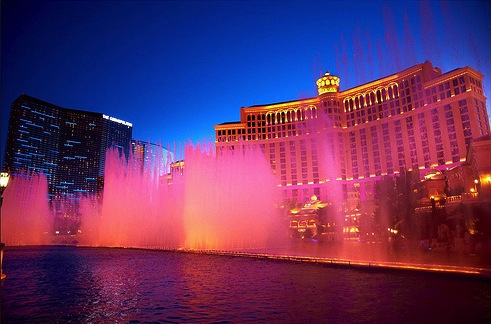
\includegraphics[width=\textwidth]{\chp3@path/3-4_random_variables/figures/bellagio.jpg}
\end{columns}
\ct{Image by Moyan\_Brenn on Flickr \webURL{http://www.flickr.com/photos/aigle\_dore/5951714693}.}
}


\end{frame}

%%%%%%%%%%%%%%%%%%%%%%%%%%%%%%%%%%%%%

\begin{frame}
\frametitle{Simplifying random variables}

Random variables do not work like normal algebraic variables:
\[ X + X \ne 2X \]

\pause

{\small
\twocol{0.45}{0.45}
{
\begin{align*}
E(X + X) &= E(X) + E(X) \\
&= 2 E(X) \\
&~  \\
E(2X) &= 2 E(X) \\
&~ 
\end{align*}
}
{
\begin{align*}
Var(X + X) &= Var(X) + Var(X)~{\scriptsize \text{(assuming independence)}} \\
&= 2~Var(X) \\
&~  \\
Var(2X) &= 2^2~Var(X) \\
&= 4~Var(X)
\end{align*}
}
}


\pause

\vspace{3mm}

\mathhl{E(X + X)  = E(2X)}, but \mathhl{Var(X + X) \ne Var(2X)}.

\end{frame}

%%%%%%%%%%%%%%%%%%%%%%%%%%%%%%%%%%%%%

\begin{frame}
\frametitle{Adding or multiplying?}

\dq{A company has 5 Lincoln Town Cars in its fleet. Historical data show that annual maintenance cost for each car is on average \$2,154 with a standard deviation of \$132. What is the mean and the standard deviation of the total annual maintenance cost for this fleet, assuming independence?}

\pause

Note that we have 5 cars each with the given annual maintenance cost $(X_1 + X_2 + X_3 + X_4 + X_5)$, not one car that had 5 times the given annual maintenance cost $(5X)$.

\pause

{\small
\begin{eqnarray*} 
E(X_1 + X_2 + X_3 + X_4 + X_5) &=& E(X_1) + E(X_2) + E(X_3) + E(X_4) + E(X_5) \\
\pause
&=& 5 \times E(X) = 5 \times 2,154 = \$ 10,770 \\
\pause
Var(X_1 + X_2 + X_3 + X_4 + X_5) &=& Var(X_1) + Var(X_2) + Var(X_3) + Var(X_4) + Var(X_5) \\
\pause
&=& 5 \times V(X) = 5 \times 132^2 = \$^2 87,120 \\
\pause
SD(X_1 + X_2 + X_3 + X_4 + X_5) &=& \sqrt{87,120} =  \$ 295.16
\end{eqnarray*}
}

\end{frame}

%%%%%%%%%%%%%%%%%%%%%%%%%%%%%%%%%%%%

\begin{frame}
\frametitle{Adding or multiplying?}

\dq{A client rents one Lincoln Town car, and their contract requires them to pay 1/5 of the maintenance cost of the car. Historical data show that annual maintenance cost for each car is on average \$2,154 with a standard deviation of \$132. What is the mean and the standard deviation of the annual maintenance cost that the client will pay?}

\pause

Note that now we have 1 car, with the annual maintenance cost $\frac{X}{5}$.

\pause 

{\small
\begin{eqnarray*} 
E\left(\frac{X}{5}\right) &=& E\left(X\times \frac{1}{5}\right) = E(X) \times \frac{1}{5} = \frac{2154}{5}  = \$ 430.8 \\
\pause
Var\left(\frac{X}{5}\right) &=& Var\left(X\times \frac{1}{5}\right) = Var(X) \times \left(\frac{1}{5}\right)^2 = \frac{132^2}{5^2} = \$^2 696.96 \\
\pause
SD\left(\frac{X}{5}\right) &=& \sqrt{696.96} =  \$ 26.4
\end{eqnarray*}
}

\end{frame}

%%%%%%%%%%%%%%%%%%%%%%%%%%%%%%%%%%%%

\begin{frame}
\frametitle{Pair work}
\dq{Given an independent sample $X_1, X_2, \ldots, X_n$, where $E[X_i]=\mu$ and $Var[X_i]=\sigma^2$. 

The sample mean is defined as:

\begin{center}$\bar{X}=\frac{1}{n}\left(X_1 + X_2 + \ldots + X_n\right)=\frac{1}{n}\sum_{1}^{n} X_i$\end{center}

What is $E[\bar{X}]$? What is $Var[\bar{X}]$? What is $StdDev[\bar{X}]$?}

\soln{
\only<2>{
\begin{eqnarray*} 
E[\bar{X}] &=& E\left[\frac{1}{n}\sum_{i=1}^{n} X_i\right] = \frac{1}{n}\sum_{i=1}^{n} E[X_i] = \frac{1}{n}\times n \times \mu = \mu \\
\pause
Var[\bar{X}] &=& Var\left[\frac{1}{n}\sum_{i=1}^{n} X_i\right] = \frac{1}{n^2}\sum_{i=1}^{n} Var[X_i] = \frac{1}{n^2}\times n \times \sigma^2 = \frac{\sigma^2}{n} \\
StdDev[\bar{X}] &=& \sqrt{\frac{\sigma^2}{n}} = \frac{\sigma}{\sqrt{n}}
\end{eqnarray*} 
}
}

\end{frame}

\begin{frame}
  \frametitle{What we just did is profound!}
  \begin{itemize}
    \item We modeled a \hl{dataset} using \hl{random variables} (Probability Theory)
    \item We defined a \hl{statistic} (the sample mean) as a \hl{function} of these random variables (the linear combination).
    \item We \emph{derived} the theoretical \hl{mean} and \hl{standard deviation} of this statistic.
    \item This is the foundation of \hl{statistical inference}, which we will cover later in the course.
  \end{itemize}
\end{frame}
%%%%%%%%%%%%%%%%%%%%%%%%%%%%%%%%%%%%

%%%%%%%%%%%%%%%%%%%%%%%%%%%%%%%%%%%%

% \section{Continuous distributions}

% %%%%%%%%%%%%%%%%%%%%%%%%%%%%%%%%%%%%

% \begin{frame}
% \frametitle{Continuous distributions}

% \begin{itemize}

% \item Below is a histogram of the distribution of heights of US adults. 

% \item The proportion of data that falls in the shaded bins gives the probability that a randomly sampled US adult is between 180 cm and 185 cm (about 5'11" to 6'1").

% \end{itemize}

% \begin{center}
% 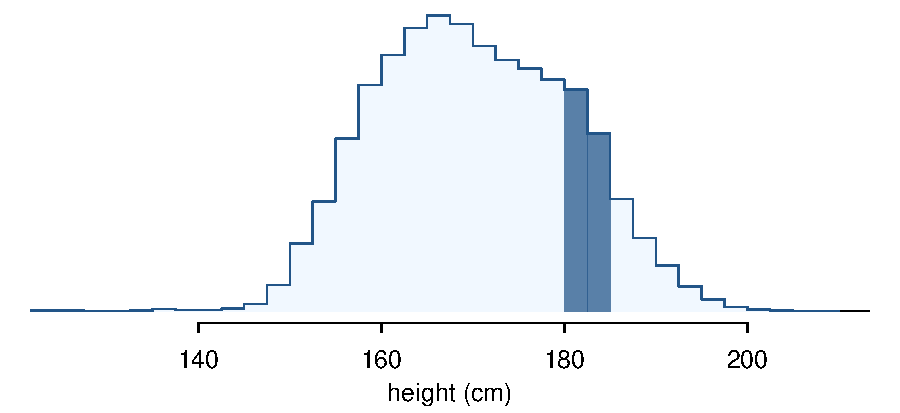
\includegraphics[width=\textwidth]{\chp3@path/3-5_continuous_distributions/figures/usHeightsHist180185/usHeightsHist180185}
% \end{center}


% \end{frame}

% %%%%%%%%%%%%%%%%%%%%%%%%%%%%%%%%%%%%

% \subsection{From histograms to continuous distributions}

% \begin{frame}
% \frametitle{From histograms to continuous distributions}

% Since height is a continuous numerical variable, its \hl{probability density function} is a smooth curve.

% \begin{center}
% 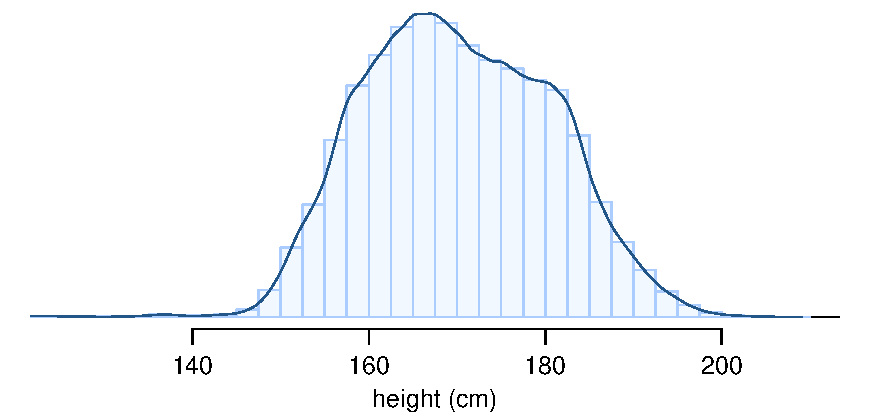
\includegraphics[width=\textwidth]{\chp3@path/3-5_continuous_distributions/figures/fdicHeightContDist/fdicHeightContDist}
% \end{center}

% \end{frame}

% %%%%%%%%%%%%%%%%%%%%%%%%%%%%%%%%%%%%

% \subsection{Probabilities from continuous distributions}

% \begin{frame}
% \frametitle{Probabilities from continuous distributions}

% Therefore, the probability that a randomly sampled US adult is between 180 cm and 185 cm can also be estimated as the shaded area under the curve.

% \begin{center}
% 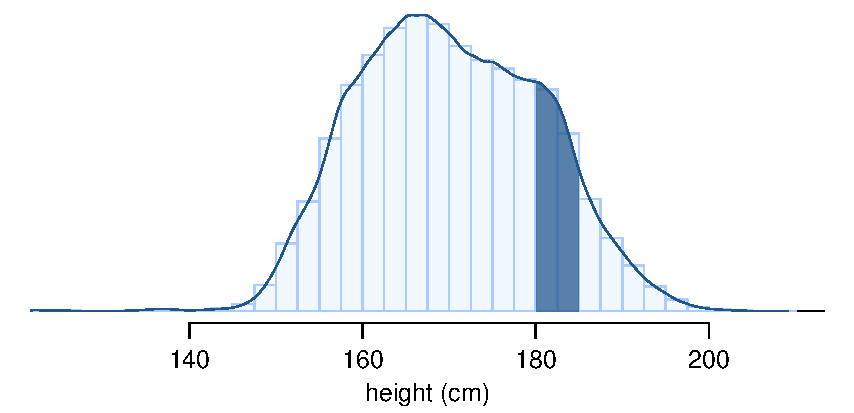
\includegraphics[width=\textwidth]{\chp3@path/3-5_continuous_distributions/figures/fdicHeightContDistFilled/fdicHeightContDistFilled}
% \end{center}


% \end{frame}

% %%%%%%%%%%%%%%%%%%%%%%%%%%%%%%%%%%%%

% \begin{frame}
% \frametitle{By definition...}

% Since continuous probabilities are estimated as ``the area under the curve", the probability of a person being exactly 180 cm (or any exact value) is defined as 0.

% \begin{center}
% 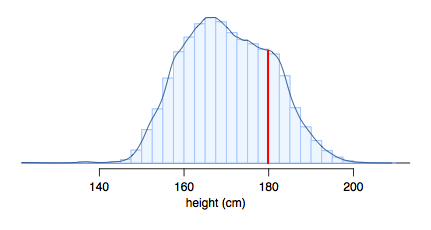
\includegraphics[width=0.8\textwidth]{\chp3@path/3-5_continuous_distributions/figures/fdicHeightContDist180}
% \end{center}

% \end{frame}

% %%%%%%%%%%%%%%%%%%%%%%%%%%%%%%%%%%%%

% \section{R Demonstration}

% %%%%%%%%%%%%%%%%%%%%%%%%%%%%%%%%%%%%

% \section{Edfinity quiz}

% %%%%%%%%%%%%%%%%%%%%%%%%%%%%%%%%%%%%

%%%%%%%%%%%%%%%%%%%%%%%%%%%%%%%%%%%%
% End document
%%%%%%%%%%%%%%%%%%%%%%%%%%%%%%%%%%%%

\end{document}